% !Tex root = main.tex
\newpage
\section{Theory}

In this section, \emph{functional dependencies} and the theoretical foundation necessary to put them into context are introduced.
Building on this foundation, \emph{relaxed functinal dependencies} are established as a way of adapting FDs for different use-cases.
Particularly \emph{robustness} of FDs will be discussed an a way of measuring it with cross-validation techniques will be presented.

Lastly, machine learning classifier theory will be discussed, introducing the \emph{Datawig} package.

\subsection{Relational Database Theory}
\emph{Functional Dependencies} (FDs) are a way of expressing ``a priori knowledge of restrictions or constraints on permissible sets of data''~\cite[p.~42]{MAI83} in relational database theory.
Introduced in the 1970s for schema normalization of relational databases, functional dependencies have proven to be useful in a multitude of domains.
In order to give a definition of FDs, they need to be put in context to the domain they stem from: relational database theory.
Some basic concepts will be introduced in this section.

\subsubsection{Relation Scheme, Relation and Tuples}
A \emph{relation scheme}\footnote{also called \emph{relational schema} in literature\cite[p.21]{ABE19} } \(\boldsymbol{R}\) is a finite set of \emph{attribute names} \( \boldsymbol{R} = \{A_1,~A_2,~\dots,~A_n\}\), where to each attribute name \(A_i\) corresponds a set \(D_i\), called \emph{domain} of \(A_i\), \(1 \leq i \leq n\).
Let \(\boldsymbol{D}~=~D_1 \cup D_2 \cup \dots \cup D_n$, then a \emph{relation} \(r\) on relation scheme \(\boldsymbol{R}\) is a finite set of mappings \(\{t_1, t_2, \dots, t_p\}\) from \(\boldsymbol{R}\) to \(\boldsymbol{D}\):
\begin{align*}
  &t_i: \boldsymbol{R} \to \boldsymbol{D}
\end{align*}
We call those mappings \emph{tuples} under the constraint that~\cite[p.2]{MAI83}
\begin{align*}
    t(A_i) \subseteq D_i.
\end{align*}
In application, attribute names are commonly called \emph{column name} or \emph{column attribute}.
One can think of them as labels of data that is stored in the respective column.


\subsubsection{Definition of a Functional Dependency}
Consider a relation \(r\) on scheme \(\boldsymbol{R}\) with subset \(X \subseteq \boldsymbol{R}\) and a single attribute \(A_i \in \boldsymbol{R}\).
A FD \(X \to A\) is said to be \emph{valid} in \(r\), if and only if
\begin{align}
    t_i[X] = t_j[X] \Rightarrow t_i[A] = t_j[A] \label{eq:fd-condition}
\end{align}
holds for all pairs of distinct tuples \(t_i,t_j \in r\).~\cite[p.~21]{ABE19}
We say that \textsc{X} \emph{functionally determines} \textsc{A}~\cite[p.~43]{MAI83} and write \textsc{X}~\( \rightarrow \)~\textsc{A}.
\(X\) is called the \emph{left hand side} (LHS) of a FD, whilst \(A\) is called the \emph{right hand side} (RHS) of the same FD.

A FD \textsc{X}~\( \rightarrow \)~\textsc{Y} is called \emph{trivial}, if \( Y \subseteq X \).\cite[p.~163]{STU16}

\paragraph{Logical Implication} Let \( F \) be the set of functional dependencies on \( \boldsymbol{R} \).
\textsc{X}~\( \rightarrow  \)~\textsc{Y} is \emph{logically implied} by \( F \), or algebraically expressed
\begin{align}
    F \models \textsc{X} \rightarrow \textsc{Y},
\end{align}
if every relational instance \( r \) of \( \boldsymbol{R} \), which satisfies all dependencies in \( F \), also satisfies \textsc{X}~\( \rightarrow \)~\textsc{Y}.~\cite[p.~166]{STU16}

Thus, if \( F = \{ \textsc{A} \rightarrow \textsc{B}, \textsc{A} \rightarrow \textsc{C}, \textsc{BC} \rightarrow \textsc{D} \} \), the following logical implications are true:
\begin{align*}
    &F \models \textsc{A} \rightarrow \textsc{B} \\
    &F \models \textsc{A} \rightarrow \textsc{BC} \\
    &F \models \textsc{A} \rightarrow \textsc{D}
\end{align*}

\paragraph{Transitive closure} Let \( F \) be a set of FDs.
The \emph{transitive closure} \( F^{+} \) of \( F \) is defined by
\begin{align}
    F^{+} := \{ \textsc{X} \rightarrow \textsc{Y} \mid F \models \textsc{X} \rightarrow \textsc{Y} \}
\end{align}

Considering table~\ref{tab:fd-example}, one can see that every tuple in the left hand side subset of the relation uniquely determines the right hand side.
We say that \textsc{Id}, \textsc{Prenameame}, \textsc{Surname}, \textsc{Town} \emph{functionally determines} \textsc{Zip} or write \{\textsc{Id}, \textsc{Prename}, \textsc{Surname}, \textsc{Town}\} \( \rightarrow \) \textsc{Zip}.~\cite[p.~43]{MAI83}

\begin{table}[ht]
    \centering
    \begin{tabular}{rlllr}
        \toprule
        & \multicolumn{3}{c}{left hand side} & \multicolumn{1}{c}{right hand side} \\ \cmidrule(lr{.25em}){1-4} \cmidrule(l{4.75em}){4-5}
        \textsc{Id} & \textsc{Prename} & \textsc{Surname} & \textsc{Town} & \textsc{Zip} \\
        \midrule
        1 & Alice & Smith & Munich & 19139 \\
        2 & Peter& Meyer & Munich & 19139 \\
        3 & Ana & Parker & Munich & 19139  \\
        4 & John & Pick & Berlin & 12055 \\
        5 & John & Pick & Munich & 19139 \\
        \bottomrule
    \end{tabular}
    \caption{Example for a FD.}\label{tab:fd-example}
\end{table}


If inspected closely, one can discover even more FDs in table~\ref{tab:fd-example}.
For example, \textsc{Town}~\( \rightarrow \)~\textsc{Zip} and \textsc{Id}~\( \rightarrow \)~\textsc{Zip}.
Since \textsc{Town} and \textsc{Id} are subsets of \{\textsc{Id},~\textsc{Prename},~\textsc{Surname},~\textsc{Town}\}, we call the FD \{\textsc{Id},~\textsc{Prename},~\textsc{Surname},~\textsc{Town}\} \( \rightarrow \)~\textsc{Zip} \emph{non-minimal}.
A FD X~\( \rightarrow \)~A is \emph{minimal}, if no subset of X functionally determines A.~\cite[p.~2]{PAP15}
Thus, \textsc{Id}~\( \rightarrow \)~\textsc{Zip} and \textsc{Town}~\( \rightarrow \)~\textsc{Zip} are \emph{minimal FDs}.

\paragraph{Full Dependency} An attribute \textsc{Y} on a relation scheme \( R \) is called \( fully dependent \) on another attribute \textsc{X} on the same scheme, if \textsc{Y} is functionally determined by \textsc{X} and \textsc{X} is minimal.~\cite[p.~61]{SCH17}
We call a \emph{determinant} a set of attributes that fully functionally determines another attribute.


\subsubsection{Keys}
\paragraph{Superkey}Let \( r \) be a relation on a relation scheme \( \boldsymbol{R} = \{ A_1, A_2, \dots, A_n \} \).
Let \( K \) be a subset of R, such that
\begin{align}
    K = \{ A_1, A_2, \dots, A_m \} \subseteq \boldsymbol{R}
\end{align}
where \( m \leq n \).
\( K \) is called \emph{superkey}, if for any tuple \( t_i \in r \) the relation
\begin{align*}
    t_i(A_k) = t_j(A_k) \Rightarrow t_i \equiv t_j
\end{align*}
holds for any single \( A_k \in K \).~\cite[p.~4]{MAI83}
In other words, if \( K \) is a superkey, any \( K \)-value of a tuple identifies that tuple uniquely.~\cite[p.~32]{SCH17}

\paragraph{Candidate key} A superkey \( K \) is called \emph{candidate key}, if it is a \emph{minimal}.~\cite[p.~32]{SCH17}
\( K \) being minimal means that \( K \) is no longer a superkey, if any attribute \( A_k \in K \) is removed from \( K \).

\paragraph{Prime Attributes} An attribute \( A \) on a relational scheme \( \boldsymbol{R} \) is called \emph{prime}, if \( A \) is part of a key of \( \boldsymbol{R} \).
Otherwise, \( A \) is called \emph{non-prime}.

\subsubsection{Definition of a Relational Database}
When real-world data used by an application is stored on a machine according to the relational model, it is usually stored in a relational database.
Following the definition of a relation scheme \( \boldsymbol{R} \), one can formally introduce databases and database schemes:

We assume that \( \boldsymbol{R}\) is composed of two parts, \(S\) and \(\boldsymbol{K}\). We call \(S\) a \emph{set of attributes} and \(\boldsymbol{K}\) a \emph{set of designated keys} and describe this composition by writing \(R = (S, \boldsymbol{K})\).
A \emph{relational database scheme} \( \mathcal{R} \) over \boldsymbol{U} can now be defined as a collection of relation schemes \( \mathcal{R} = \{R_1, R_1, \dots, R_p\} \), where \(R_i = (S_i, \boldsymbol{K}_i)\), \(1 \leq i, j \leq p\),
\begin{align*}
    \boldsymbol{U} := \bigcup^{p}_{i=1} S_i
\end{align*}
We demand that \(S_i \neq S_j\) if \(i \neq j\).

A \emph{relational database} \( d \) on a \emph{database scheme} \( \mathcal{R} \) is a collection of relations \( d~=~\{r_1, r_2, \dots, r_p \} \) such that for each relation scheme \(R = (S, \boldsymbol{K}) \) in \( \mathcal{R} \) there is a relation \(r\) in \(d\) such that \(r\) is a relation on \(S\) that satisfies every \emph{key} in \(\boldsymbol{K}\).~\cite[p.~94]{MAI83}


\subsection{FDs in Application}
FDs are primarily used in database normalization.~\cite[p.~1]{CAR16}
In 1970, Codd defined the \emph{relational model}~\cite{COD70} and pioneered many important concepts in database theory.
In the following paragraphs, selected sections of Codd's work will be introduced to put FDs into context.

\subsubsection{Normalization}
When introducing the relational database model in his 1970 article ``A relational model of data for large shared data banks'', Edgar F. Codd formalized database normalization alongside.~\cite{COD70}
Describing what will be know to academia as \emph{first normal form} (1NF), Codd states that ``problems treated [when normalizing databases] are those of \emph{data independence}'', aiming to protect future users of large databases ``from having to know how the data is organized in the machine''.~\cite[p.~1]{COD70}

Databases at the time were structured hierarchically or navigationally.
This design was centered on efficiency, aiming for query handling as fast as possible.
While this design yielded good performance in an era when computing time was cost-intensive, it came with a heavy cost of complexity:
``Teams of programmers were needed to express queries to extract meaningful information. [\dots] Such databases [\dots] were absolutely inflexible[y]''.~\cite{IBM03}

Codd's relational model shifted the focus of database architecture away from efficiency and towards a new, more user-centered design.
Among its many benefits compared to previous database designs was
Update-, insertion- and deletion anomalies can be prevented when normalizing a relational database.~\cite[p.~75]{KLE11}

\paragraph{First Normal Form} A relation scheme $R$ is in \emph{First Normal Form} (1NF), if values in \(dom(A)\) are atomic for every attribute \(A\) in \(R\).~\cite[p.~96]{MAI83}
Consider table~\ref{tab:first-normal-form} which represents two relational database schemes.
It serves as an example of what is called atomic- and compound data in the Relational Database model.~\cite[p.~6]{COD90}

\begin{table}[ht]
    \centering
    \ra{1.3}
    \begin{tabular}{rlllllll}\toprule
    & \multicolumn{3}{c}{Compound Scheme} & & \multicolumn{2}{c}{Atomic Scheme} \\
    \cmidrule{2-3} \cmidrule{5-8}
    & \textsc{Name} & \textsc{Adress} && \textsc{Prename} & \textsc{Surname} & \textsc{Town} & \textsc{Street}   \\ \midrule
1 & Alice Smith & Munich, Flurstr. && Alice & Smith & Munich & Flurstr. \\
2 & Peter Smith & Munich, Flurstr. && Peter & Smith & Munich & Flurstr. \\
3 & Ana Parker & Munich, Anastr. && Ana & Parker & Munich & Anastr. \\
4 & John Pick & Berlin, Flurstr. && John & Pick & Berlin & Flurstr. \\
\bottomrule
\end{tabular}
\caption{The compound attributes \textsc{Adress} and \textsc{Name} can be split into their atomic components \textsc{Town} and \textsc{Street} as well as \textsc{Prename} and \textsc{Surname}, respectively.}\label{tab:first-normal-form}
\end{table}
While the compound scheme's attributes can be decomposed into several other attributes, whereas an atomic attribute cannot be further split into any meaningful smaller components.

For a database it is said that the database in 1NF if every relation scheme in the database scheme is in 1NF.
1NF is the very foundation of the Relational Model, where the only type of compound data is the relation.~\cite[p.~6]{COD90}

\paragraph{Second Normal Form (2NF)} A relation scheme \(R\) is said to be in \emph{second normal form} (2NF) in respect to a set of FDs \(F\), if it is in 1NF and every nonprime attribute is fully dependent on every key of of \(R\).~\cite[p.~99]{MAI83}
This definition can be extended for databases: A database scheme \textbf{R} is in second normal form with respect to \(F\) if every relation scheme \(R\) in \textbf{R} is in 2NF with respect to \(F\).

\paragraph{Boyce-Codd Normal Form (BCNF)}
A relation scheme \( R \) is in \emph{Boyce-Codd Normal Form}, if every determinant in \( R \) is a candidate key.~\cite[p.~65]{SCH17}


\subsection{Limitations of FDs}
In the field of dependency detection an extensive body of theory and algorithms for FD detection has been created in the past decades.\cite[p.~1]{PAP15}
These mainly consider FDs as defined in formula~\ref{eq:fd-condition}.
Howevever, the strict detection of FDs yields results that are solely applicable in a strictly controlled environment.

Real-world datasets that researchers, data scientists or database engineers work with are often \emph{noisy}.
This noise has many faces:
Entries might be corrupted by missing data, wrongly entered data or incomplete data.
Columns might contain data of different kind, where one column could contain the binary representation of an image and another column the contains of a wave-audiofile.
In these cases, functionally dependent column-combinations might not be detected as such.
This may result in misleading insights when searching for FDs.

Researchers have faced these limitations of FDs in the past in many domains.
This lead to the definition of many new kinds of dependencies.
While there are RFDs introducing general error measures, others are defined ``aiming to solve specific problems''\cite[p.~147]{CAR16}.
Since all of these \emph{new} kinds of dependencies relax the conditions in equation~\ref{eq:fd-condition}, they are called \emph{relaxed functional dependencies (RFDs)}.
Caruccio et al.\ classified and compared 35 different RFDs~\cite[p.~151]{CAR16}.

In order to classify RFDs, Carucio et al.\ state that each RFD was ``based on its underlying relaxation criteria''\cite[p.~149]{CAR16}.
They proceed to define two such relaxation criterions.
\emph{Attribute comparison} refers to ``the type of tuple comparison used on the LHS and RHS''.
The relaxation criterion \emph{extent} describes a relaxation of the set of tuples for which a FD is valid.

\subsubsection{FDs relaxing on the Extent}
The term \emph{extent} is used to describe how a RFD relaxes on the subset of tuples for which the RFD is satisfied.

\begin{figure}[ht]
     \centering
     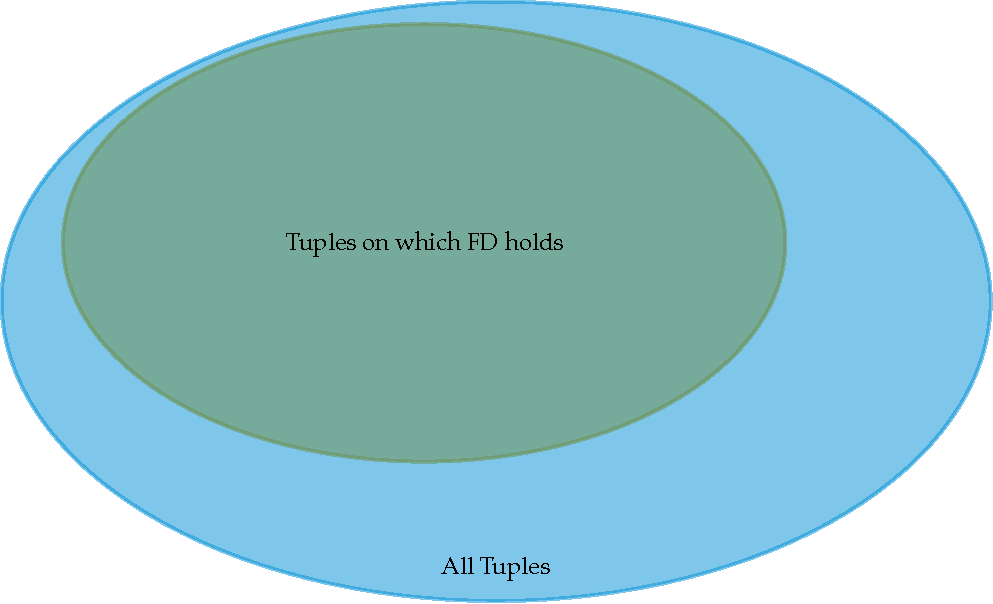
\includegraphics[width=.4\textwidth]{images/rfds-extent.pdf}
     \caption{Venn diagram representing the extent relaxation criteria.}
     \label{fig:rfds-extent}
 \end{figure}

RFDs implement this idea in different ways.
In the following section, a selection of RFDs relaxing the extent of the FD will be briefly presented.

\paragraph{Approximate Functional Dependency (AFD)}
AFDs improve the applicability of FDs, by ``holding on almost every tuple''\cite[p.~151]{CAR16}.
An To illustrate this, table~\ref{tab:example-afd-necessity} shows an example of noisy data.
The potential FD \textsc{Town} \(\to\) \textsc{Zip} is not captured by the definition given in equation~\ref{eq:fd-condition}.
Due to a type-error, the potential FD is invalidated.
To still capture meta-information, a different dependency-measure than given in equation~\ref{eq:fd-condition} is needed.

\begin{table}[ht]
    \centering
    \begin{tabular}{lcccc}
        \toprule
        & \multicolumn{3}{c}{Data} \\ \cmidrule(lr){2-5}
        \textsc{Id} & First name & Last name & Town & \textsc{Zip} \\
        \midrule
        1 & Alice & Smith & Munich & 19139 \\
        \textbf{2} & \textbf{Peter}& \textbf{Meyer} &
        \textbf{Muinch} & \textbf{19139} \\
        3 & Ana & Parker & Munich & 19139  \\
        4 & John & Pick & Berlin & 12055 \\
        \bottomrule
    \end{tabular}
    \caption{Even though column \textsc{Zip} functionally determines column \textsc{Town} (and vice-versa), a FD is not capable of displaying this fact~-~a typing error invalidates the FD.}
    \label{tab:example-afd-necessity}
\end{table}

Tuples that do not correspond to the canonical FD are measured as fraction of the total of tuples on a relation \( r \) as follows:

\begin{align}
    \Psi(X, Y) = \frac{\min{\left(|r_1|~|~r_1 \subseteq r \text{ and } \textsc{X} \rightarrow \textsc{Y} \text{ hold in } r \setminus r_1 \right)}}{|r|}
\end{align}

Here, function \( \Psi(X, Y) \) is called \emph{coverage measure} of a RFD \textsc{X} \( \to \) \textsc{Y}.
\( \Psi \) ``quantifies the satisfiability degree of an RFD [\dots] on \( r \)''\cite[p.~150]{CAR16} and is used in the definition of an AFD to be compared to a threshold \( \epsilon \in [0, 1] \).

If \( \Psi(X, Y) \) is smaller or equal to \( \epsilon \), the AFD is said to hold on a relation \( r \).
Applied to table~\ref{tab:example-afd-necessity}, the AFD \textsc{Town} \( \to \) \textsc{Zip} holds, if \( \epsilon \geq 0.25\).

\paragraph{Conditional Functional Dependencies (CFDs)}
\emph{Conditional Functional Dependencies} employ conditions to define the subset on which a dependency holds.
Originally, those conditions exclusively allow the definition of constraints using the equality operator.\cite[p.~152]{CAR16}
Applied to table~\ref{tab:example-afd-necessity}, a CFD \textsc{Town} \( \to\) \textsc{Zip} holds under the condition that a) entries in column \textsc{Town} = Munich or b) entries in column \textsc{Town} = Berlin.

Other RFDs based on the definition of CFDs include \emph{extended conditional functional dependencies} (ECFDs) by Bravo et al.\ that allow the disjunction-operator as well as the inequality-operator for defining conditions.\cite{BRA08}

Also, Chen et al.\ defined CFD\textsuperscript{p}s, which introduce \( <, \leq, >, \geq \text{and} \neq \) for defining conditions.\cite{CHE09}

\subsubsection{FDs Relaxing on the Attribute Comparison}
Instead of specifying subsets of tuples for which a FD is valid, FDs relaxing on the attribute comparison alter the condition under which a dependency is said to be valid.

\paragraph{Metric Functional Dependencies (MFDs)}
First introduced by Koudas et al.\ in 2009, \emph{Metric Functional Dependencies} were defined to adress violations of canonical FDs due to ``small variations [\dots] in data format and interpretation''.\cite[p.~1]{KOU09}

According to equation~\ref{eq:fd-condition}, a FD \textsc{Town} \( \to\) textsc{Zip} is said to be valid if
\begin{align}
    t[\textsc{Town}] = t'[\textsc{Town}] \Rightarrow t[\textsc{Zip}] = t'[\textsc{Zip}]
\end{align}
holds for all pairs of distinct tuples \( t_i, t_j \in r \), where \( r \) is a relation on scheme \( \boldsymbol{R} \).
The definition of a MFD replaces this equation by demanding that if and only if for all pairs of distinct tuples \( t_i, t_j \in r \) the metric condition
\begin{align}\label{eq:mfd-condition}
    t[\textsc{Town}] = t'[\textsc{Town}] \Rightarrow d(t[\textsc{Zip}], t'[\textsc{Zip}]) \leq \delta
\end{align}
holds, the MFD \textsc{Town} \( \to\) \textsc{Zip} is said to be valid on \( r \).\cite[p.~2]{KOU09}
Here, \( \delta \) is called a \emph{tolerance parameter}, indicating how far the result of a \emph{metric} \( d(t[\textsc{Y}], t'[\textsc{Y}]) \) can deviate from exact equality.

One such metric \( d \) would be the absolute difference between two values, such that \( d(t[\textsc{Y}], t'[\textsc{Y}]) = | t[\textsc{Y}] - t'[\textsc{Y}]| \).
Another popular metric for measuring the difference between two sequences is the Levenshtein distance, where \( d(t[\textsc{Y}], t'[\textsc{Y}]) = \text{lev}_{t,t'}(|t|, |t'|) \) and
\begin{align*}
    \text{lev}_{t,t'} =
    \begin{cases}
        \max(i,j),  & \text{if} \min(i,j)=0, \\
        \min \begin{cases}
            \text{lev}_{a, b}(i-1, j)+1 & \\
            \text{lev}_{a, b}(i, j-1)+1 & \\
            \text{lev}_{a, b}(i-1, j-1)+1_{(a_i \neq b_j)} \\
        \end{cases} & \text{otherwise.}
    \end{cases}
\end{align*}
Regarding the example given in table~\ref{tab:example-afd-necessity}, the Levenshtein distance between \texttt{Munich} and \texttt{Muinch} is 2.
Thus the MFD \textsc{Town} \( \to\) \textsc{Zip} is valid, if \( d = \text{lev} \) and \( \delta = 2 \).

\paragraph{Purity Dependencies (PUDs)}
\emph{Purity Dependencies} Lorem ipsum

\subsection{Robustness of FDs}
When Edgar F. Codd introduced the relational model in 1970, the concept of keys and thus the concept of functinal dependencies was already present.\cite[p.~70]{MAI83}
However, in 1972 Codd separated the definition of a FD from keys, persuing the specific goal of normalizing a relational database scheme.
In the years to follow, different researchers started using FDs in their works to solve problems other than schema normalization.

Koudas et al., when introducing the MFD, write that the definition of FDs was ``not \emph{robust}\footnote{Highlighting added by the author.} enough to capture functional relationships on data obtained from merging heterogenous sources [\dots]''.\cite[p.~1]{KOU09}
However, they do not provide a way of measuring robustness.

Bleifuß et al.\cite[p.~3]{BLE16} define \emph{Correctness} of a set of RFDs \( Out \) compared to a set of FDs \( Gold \) on the same relational instance \( r \) as follows:
\begin{align*}
    \text{Correctness} = \frac{|Out \cap Gold^{+}|}{|Out|}
\end{align*}
\( Gold^{+} \) represents the transitive closure of \( Gold \), meaning that it includes all non-minimal FDs implied by \( Gold \).
However, this definition is only meaningful for AFDs, which try to minimc FDs as closely as possible.

As far as the author of this work knows, there is no method for measuring \emph{robustness} of FDs established.
Drawing inspiration from Machine Learning theory, we propose the application of cross-validation techniques to functional dependencies in order to measure robustness, as it has been described by Koudas et al.\, in a meaningful way.

\subsubsection{Measuring Robustness}
Let \( r = \{ t_1, t_2, \dots, t_p \}\) be a a relation on a relation scheme \( \boldsymbol{R} \).
Then \( p \in \mathbb{N} \) is the number of tuples in \( r \).
We then introduce a split-ratio \( s \in (0, 1) \) and split \( r \) into two subsets:
\begin{align*}
    r_{train} &= \{ t_1, t_2, \dots, t_{s \cdot p} \} \\
    r_{test} &= \{ t_{(s \cdot p) + 1}, t_{(s \cdot p) + 2}, \dots, t_{p} \}
\end{align*}
If \( s \cdot p \) is not a natural number, we round accordingly.
We call \( r_{train} \) the \emph{train set} and \( r_{test} \) the \emph{test set}.
In table~\ref{tab:split-example-fd-imputer} such a splitting is examplified for \( s = 0.5 \) and \( p=4 \).
This approach is drawn from statistical cross-validation.

\begin{table}[ht]
    \begin{subtable}[c]{0.9\textwidth}
        \centering
        \begin{tabular}{llll}
            \textsc{A} & \textsc{B} & \textsc{C} & \textsc{D} \\
        \toprule
        Blue & Car & Portugal & Lisbon \\
        Yellow & Car & Portugal & Lisbon  \\
        Green & Bus & Spain & Madrid  \\
        Grey & Car & Portugal & Lisbon  \\
        \bottomrule
        \end{tabular}
        \subcaption{Original relation \( r \).}
    \end{subtable}
    \begin{subtable}[c]{0.45\textwidth}
        \centering
        \begin{tabular}{llll}
            \textsc{A} & \textsc{B} & \textsc{C} & \textsc{D}  \\
        \toprule
            Green & Bus & Portugal & Lisbon \\
            Yellow & Car & Portugal & Lisbon \\
        \bottomrule
        \end{tabular}
        \subcaption{Train set \( r_{train} \).}
    \end{subtable}
    \begin{subtable}[c]{0.45\textwidth}
        \centering
        \begin{tabular}{llll}
        \textsc{A} & \textsc{B} & \textsc{C} & \textsc{D} \\
        \toprule
        Yellow & Bus & Spain & Madrid \\
        Blue & Bus & Portugal & Lisbon \\
        \bottomrule
        \end{tabular}
        \subcaption{Test set \( r_{train} \).}
    \end{subtable}
    \caption{The relation \( r \) is split into train- and test sets with a split-ratio \( s = 0.5 \). }
    \label{tab:split-example-fd-imputer}
\end{table}

In a next step, FDs are detected on the train set using the HyFD algorithm.\cite{PAP16}
The algorithm we call \emph{FD Imputer} is then used for measuring robustness of each FD detected on the train set.

\paragraph{FD Imputer} FD Imputer iterates through each tuple in the test set and searches for a tuple in the train set with the exact same left hand side.
If one or more such tuples in the train set are found, FD Imputer randomly selects one of these tuples and saves the right hand side of that tuple.
We call this right hand side value \emph{imputation} of the right hand side value on the train set.

This is done for all tuples in the train set.
In a last step, FD Imputer compares the imputations with the actual right hand side values in the train set.
This allows a classification of the imputations --- one can now calculate the F1-measure for each FD.

Consider table~\ref{tab:split-example-fd-imputer}.
The FD \textsc{C} \( \ \to \) \textsc{D}, when used for finding a right hand side value on \( r_{test} \), will correctly return `Lisbon'.
However, FD \textsc{A} \( \to \) \textsc{D} for example will lead to FD Imputer yielding `Madrid', which is an incorrect imputation.

Implementing FD Imputer, imputations are retrieved by executing a SQL join clause.
FD Imputer performs an inner join on all left hand side columns, joining train-set and validation-set.
A successive second left join clause concatenates the original validation-set with the column of imputed tuples stemming from the first join.

\paragraph{Robustness as a F1-Score} The imputed values retrieved by FD Imputer can be leveraged to create a measure for robustness.
Each imputed value is interpreted as a label and classified as in the binary classification case (see figure~\ref{fig:confusion-matrix}).
Precision and recall are then calculated and weighted according to the number of true instances for each label.\footnote{See \href{https://scikit-learn.org/stable/modules/generated/sklearn.metrics.f1_score.html}{sklearn documentation} for \texttt{sklearn.metrics.f1\_score()} with weighted average.}

Finally, this approach yields a f1-score for each FD which we call \emph{robustness}.

\newpage

\subsection{Machine Learning Classifier Theory}
Once a model has been trained and validated, it needs to be tested in order to determine whether or not overfitting occured during training.
This is usually done by measuring the model's performance on a separate dataset not involved in training, the so called test set.
Performance is measured according to the type of data and the kind of model involved.
To visualize the performance of a classifier, a \emph{confusion matrix} can be created.
\begin{figure}[ht]
     \centering
     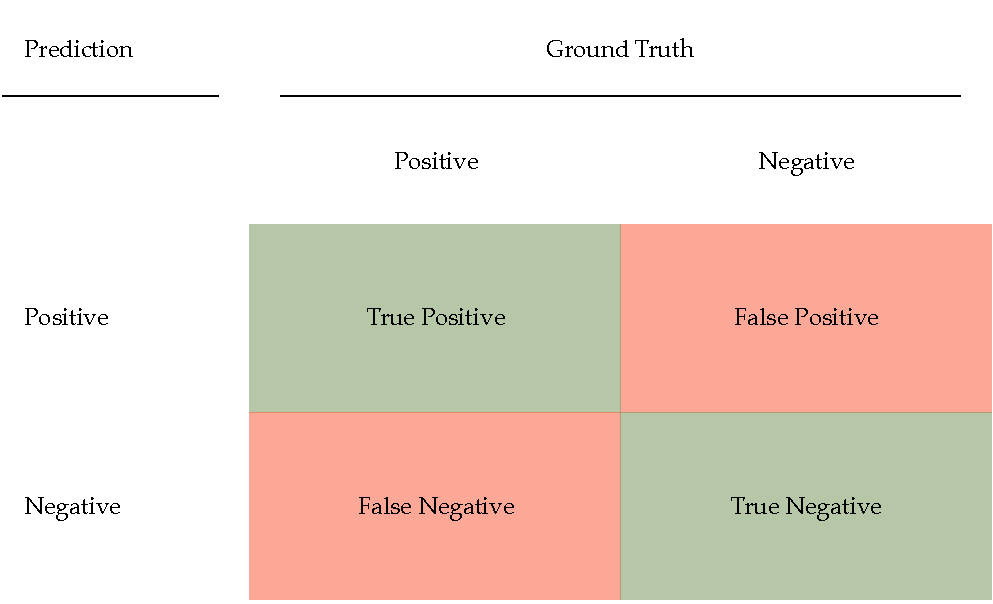
\includegraphics[width=.8\textwidth]{images/binary-confusion-matrix.pdf}
     \caption{Illustration of a binary confusion matrix.
     ``Prediction'' refers to predicted labels \(y_{pred}(x)\) while ``Ground Truth'' represents the actual labels \(y(x)\).}
     \label{fig:confusion-matrix}
 \end{figure}

The simplest case of a confusion matrix can be created when measuring the performance of a binary classifier.
Figure~\ref{fig:confusion-matrix} shows such a binary confusion matrix.
Here, ``Ground Truth'' describes the label \(y(x)\) of some data point \(x \in X_{test}\), where \(y \in \{0, 1\}\).
``Prediction'' identifies the predicted labels \(y_{pred}(x)\) that the model generates after is has been executed on the test-set \(X_{test}\) prior unknown.

Whenever \(y_{pred}(x) = y(x),~x \in X_{test}\) holds, the predicted label can be assigned to be either a \emph{True Positive} (TP) or a \emph{True Negative} (TN).
The opposite holds as well, such that a falsely predicted label will be either a \emph{False Negative} (FN) or a \emph{False Positive} (FP).

Using the classification introduced by the binary confusion matrix, all predicted labels \(y_{pred}\) are assigned to the four sets TP, TN, FN and FP.
Using these four sets, we can introduce measures for classification performance.

\emph{Precision} is a measure that depicts the proportion of correctly classified positive samples to the total amount of samples classified as positive.\cite[p.4]{THA18} This can be algebraically expressed as
\begin{align}
    Precision = \frac{|TP|}{|TP| + |FP|}
\end{align}
where \(|A|\) is the cardinality of a set \(A\). Precision measures how many elements classified as positive are True Positives.

\emph{Recall}, also called \emph{sensitivity}, represents the
share of positive correctly classified samples to the total amount of positive samples.\cite[p.3]{THA18} This can be formalized as
\begin{align}
    Recall = \frac{|TP|}{|TP| + |FN|}
\end{align}
Recall measures how many of the positive labelled elements were actually selected.

\begin{figure}[ht]
    \centering
    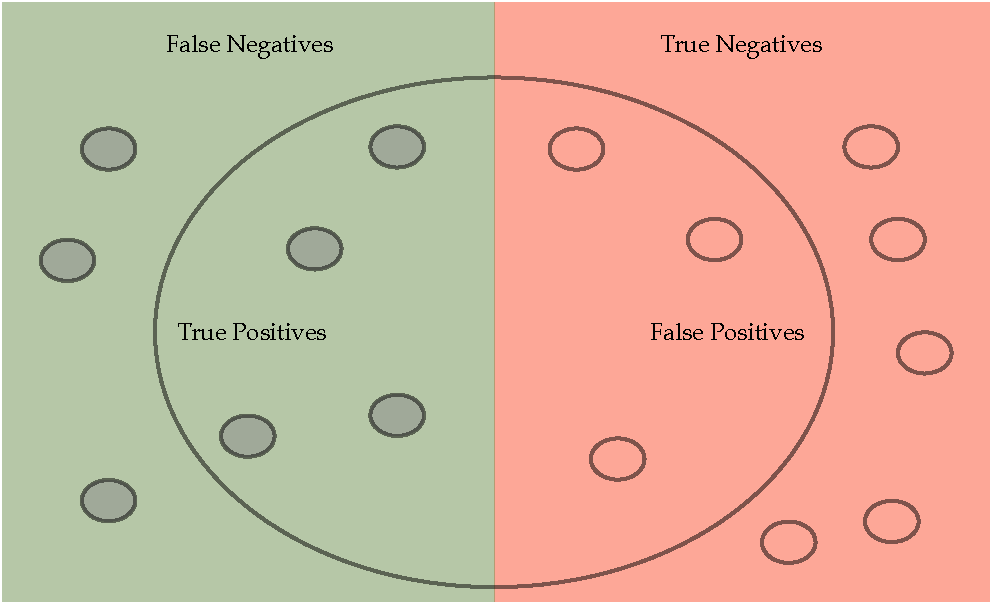
\includegraphics[width=.5\textwidth]{images/precision-and-recall}
    \caption{Each predicted label \(y_{x}\) is represented by a circle. Hollow circles stand for negative labels and full circles for positive lables.  }
    \label{fig:precision-and-recall}
\end{figure}

The harmonic mean of precision and recall is called \emph{F1-measure}:
\begin{align}
F1-measure = {\left(\frac{Recall^{-1} + Precision^{-1}}{2}\right)}^{-1}
\end{align}

\subsubsection{Datawig Imputer}
Datawig Imputer is an imputation method based on \emph{supervised learning}.
In supervised learning, observations are a set of tuples \( \{\left(\mathbold{x}_1, y_1\right),\left(\mathbold{x}_2, y_2\right), \dots \} \).
We call \( \mathbold{x}_i \in \mathbb{F}\) \emph{feature-vector} in a \emph{feature-space} \( \mathbb{F} \subseteq \mathbb{R}^{n} \) and \( y_i \in S \) \emph{output-attributes} or \emph{labels}.\cite[p.19]{DUD00}

Datawig Imputer solves a classification problem.
A function
\begin{align}
    f: \mathbb{F} \rightarrow S
\end{align}
is being approximated, where \( \mathbb{F} \) is the feature-space and \( S = \{a_1, a_2, \dots, a_M \} \) is a set of attributes.

Datawig Imputer assumes that the column to be imputed, the so-called \emph{label comumn}, contains data that can be transform to obtain attributes \( a_1, \dots, a_M \).\cite[p.2]{BIE18}
All columns on a database table that are \emph{not} the label column are called \emph{feature columns}.
These feature columns are what Datawig Imputer will transform to obtain feature-vectors.

The transformation performed to obtain learnable data assign to the \texttt{string} data of each column \( c \) a numerical representation \( x^c \).
These functions are called \emph{encoders}.
Datawig Imputer separates data into two categories: \emph{categorical data} and \emph{sequential data}.
Different encoders are chosen to transform \emph{categorical data} and \emph{sequential data}.

Categorical data are data that consist of \emph{categorical variables}.
``A categorical variable places a case into one of serveral groups of categories,{''} define Moore et al.\cite[p.~4]{MOO11}
An example-column \( c_{cat} \) containing categorical variables can be representend by the following set of colors:
\begin{align}\label{eq:c-cat}
    c_{cat} = \{ \texttt{blue},~\texttt{red},~\texttt{yellow},~\texttt{blue},~\texttt{blue},~\texttt{red} \}
\end{align}
Datawig Imputer creates a histogram of column \( c \) and uses the histogram's index \( x^c \in \{1, 2, \dots, M_c \} \) to generate a numerical representation.
\begin{figure}[ht]
    \centering
    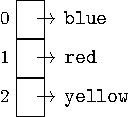
\includegraphics[width=.3\textwidth]{images/state_diagrams/color_histogram}
    \caption{State diagram showing the histogram established by Datawig Imputer to encode example~\ref{eq:c-cat}}
    \label{fig:state-diagram-color}
\end{figure}
Thus the encoded column \( c_{cat} \) would have the following form:
\begin{align}
    c_{cat}^{c} = \{ 0, 1, 2, 0, 0, 1\}
\end{align}

Sequential data is data where the sequece in which individual datapoints are stored in contains information.
An example for sequential data would be a column containing non-categorical strings, like Usernames:

\begin{align}
    c_{seq} = \{ \texttt{ItalyPaleAle},~\texttt{sisou},~\texttt{primos63} \}
\end{align}

The numerical representation \( c_{seq}^{c} \in \{ 0, 1, 2, \dots, A_c \}^{S_c} \) of the sequential column ``is a vector of length \( S_c \), where \( S_c \) denotes the length of the sequence or \texttt{string} in column \( c_{seq} \).''\cite[p.2020]{BIE18}
This numerical representation is called \emph{n-gram representation}.
For further details on the n-gram implementation, consider~\cite[p.2020]{BIE18}.

Finally, the Datawig-Imputer learns to predict the label distribution from \( y \in {1, 2, \dots, D_y} \) from the feature-vector \( \mathbold{x} \).
It therefore models \( p(y|\mathbold{x},\mathbold{\Theta}) \), the \( D_y \)~-~dimensional probability vector over all possible values in the to-be imputed comumn in function of feature-vector \( \mathbold{x} \) and \emph{learned model parameters} \( \mathbold{\Theta} \).
Datawig uses a simple logistic regression type output layer to achieve this:
\begin{align}
    p(y|\mathbold{x},\mathbold{\Theta}) = \texttt{softmax}[\mathbold{Wx} + \mathbold{b}]
\end{align}
Here, the learned model parameters \( \mathbold{\Theta} = (\mathbold{W}, \mathbold{z}, \mathbold{b}) \) depends on the learned \emph{weights} \( \mathbold{W} \) and \emph{biases} \( \mathbold{b} \) as well as \( \mathbold{z} \), representing all parameters of the column-specific feature extraction.
Parameters \( \mathbold{\Theta} \) are learned by minimizing cross-entropy loss between predicted and observed labels \( y \) by computing
\begin{align}
    \mathbold{\Theta} = \min_{\Theta} \sum\nolimits_{1}^{N} - \log(p(y|\mathbold{x}, \mathbold{\Theta}))^\top \texttt{onehot}(y).
\end{align}
Here, \( \log() \) represents the element-wise logarithm.
\( \texttt{onehot}(y) \in {0, 1}^{D_y}\) stands for a one-hot encoding of one label \( y \).

Training is done using standard backpropagation and stochastic gradient-descent on mini-batches.
The exact network layout is described in the paper ``Deep Learning for Missing Value imputation in Tables with Non-Numerical Data''~\cite[p.2022]{BIE18} in full detail.


